\chapter{Results and Discussion}
\label{results}

\section{Data Preprocessing and Network Construction}
The issue with combining different data sources is that sometimes they are inconsistent and/or incomplete, which is why data preprocessing is needed to create a sufficient network that can be used to prediction tasks. However, preprocessing of data can also mean the loss of incompatible yet important information. The main preprocessing task in this thesis was the merging of chemicals from the \ac{SIDER} and DrugBank graphs, although both graphs contained chemicals that were labeled with PubChem identifiers, some chemicals can have two or more PubChem identifiers, that can contain different stereochemistry or isotopes of the same compound. This resulted in having different nodes of the same chemical from the two different databases, which meant that the model would not be able to correctly predict relations for this chemical because they not complete. To resolve this issue, the nodes of the chemicals were merged using their canonical \ac{SMILES}, which focuses on the topology of the compound and disregards its stereochemistry. However, another issue could emerge from this approach, since isomers from the same compound do not always elicit the same response, which could cause a different kind of problem in the predictions.
The network was built first using two databases, \ac{SIDER} and DrugBank, which contained three types of nodes, chemicals, phenotypes, and targets, and two types of relations, chemical - phenotype, and chemical - target, in total. However, this was not enough to build a graph that is able to predict new relations, since it would not have enough relations to learn from. This is why chemical similarity, chemical - chemical, relations were added to the complete graph.

\section{Model Evaluation and Selection}
Six different \ac{NRL} models were selected based on their approaches; two of the methods were matrix factorization-based, \ac{HOPE} and \ac{GraRep}, two used deep learning approaches, \ac{LINE} and \ac{SDNE}, and two methods were random walk-based, DeepWalk and node2vec. All different approaches were evaluated and the approach that works best with the data set created for this thesis was selected. Translational distance-based models, TransH and TransR, were also trained and evaluated, however, they performed poorly on this kind of biological network. This might be because the network created for this thesis contains a large number of relations compared to the entities. Moreover, this network contains unbalanced relationships, e.g. many-to-one, one-to-many, and many-to-many, which might create a challenge for translational models to map n-side entities to suitable positions in the embedding space \cite{liang_predicting_2019}.

Biological networks are usually sparse, noisy, and incomplete \cite{nickel_review_2016}, leading to challenges in identifying and understanding structures, patterns, and dynamics of the network \cite{wang_unsupervised_2016}. Furthermore, they can be heterogeneous and high dimensional, making the embedding task much more complicated. Hence, understanding the topology of the network to be analyzed is important to decide the preserved structural properties in the embeddings. In the case of biological networks, preserving both local and global structural properties seem to be the most fitting for a better analysis of the network \cite{su_network_2018}. This is true because biological networks are complex and usually contain essential information both locally and globally. Thus, the \ac{NRL} models were selected based on the fact that they can capture the local and global structures of the network to insure that they perform well enough.

\subsection{Trained Graph Selection}
Both the complete graph with 50\% similarity relations and the complete graph with clusters relations were tried, and both performed well. However, the graph with 50\% similarities produced a lot of predictions that do not make sense, which could be related to the fact that the threshold for making an edge between two chemicals was low, creating many unnecessary relations that could contribute to a inaccurate prediction. The graph could have performed well because of its high inter-connectivity, which means that there is a high chance that an edge exists between any two given nodes. Thus, the complete graph with clusters relations was chosen for training and prediction.

All the models went through 100 trials, hyperparameters were randomly selected at each run. For each method, a set of parameters that play a role in the embeddings generation were selected to be optimized. All the models, with the exception of SDNE, have embeddings dimensions, which is an important paramter to optimize since it will contain all the low-dimensional representations of the graph. In GraRep, $k$-step parameter indicates length of the longest path that the embeddings will contain. The selection of order in \ac{LINE} determines if the model will preserve the local structure (order=1), global structure (order=2), or both (order=3). The epochs in \ac{LINE} and \ac{SDNE} control the number of times the model will go through the training set. $\alpha$ and $\beta$ parameters determine the proximity and reconstruction weight, respectively, as mentioned previously in \ref{subsection:SDNE}. Random walk methods, DeepWalk and node2vec, use the walk length to control length of path, number of walks to determine how many paths each node has, and the window size which determines the number of nodes that are captured on either sides of the target node.

The training set was used to generate the embeddings for each \ac{NRL} model and to train the logistic regression, then the model was evaluated using testing set. The best trial for each model was selected based on the highest \ac{MCC} score. This metric was chosen for the optimization because it is an unbiased and balanced measure that works on both balanced and unbalanced data sets, thus it is a more stable measure of performance.

Table \ref{tab:evaluation_results} presents the parameters and evaluation metrics for the best trial of each method. All models, with the excpetion of \ac{SDNE}, performed faily well, with AUC-ROC and AUC-PR of above 0.9, and MCC of above 0.8, however the model that performed the best was node2vec with AUC-ROC of 0.977, AUC-PR of 0.981, and \ac{MCC} of 0.877, which is why it was chosen to be the model used for prediction. All performance results are presented in Table \ref{tab:evaluation_results}. node2vec model worked best for this data set because of the hyperparameters selected. A window size of 4 and walk length of 8 were big enough to include nearby nodes and paths to learn and predict nodes that are not directly related (target - phenotype associations), but not too big as to include unnecessary or relations. The number of walks made sure to learn the paths between nodes without overfitting the network so new predictions can be made. Furthermore, high $p$ and $q$ parameters ensured that the model would avoid revisting nodes yet it would be biased toward nodes that are closer to the previous node, which helped in capturing the local and global structures of the network.

\begin{table}[h!]
    \centering
    \small
    \begin{tabular}{ |l|l|r|r|r|r| } 
        \hline
        \textbf{Method} & \textbf{Parameters} & \textbf{Value} & \textbf{AUC-ROC} & \textbf{AUC-PR} & \textbf{\ac{MCC}} \\
        \hline
        \multirow{6}{*}{node2vec} & Dimensions & 300 & \multirow{6}{*}{\textbf{0.977}} & \multirow{6}{*}{\textbf{0.981}} & \multirow{6}{*}{\textbf{0.877}} \\ 
            & Walk length & 8 & & & \\
            & Number of walks & 8 & & & \\
            & Window size & 4 & & & \\
            & Return parameter ($p$) & 2.3 & & & \\
            & In/out parameter ($q$) & 1.9 & & & \\
        \hline
        \multirow{4}{*}{DeepWalk} & Dimensions & 300 & \multirow{4}{*}{0.969} & \multirow{4}{*}{0.974} & \multirow{4}{*}{0.846} \\
            & Walk length & 8 & & & \\
            & Number of walks & 8 & & & \\
            & Window size & 2 & & & \\
        \hline
        HOPE & Dimensions & 300 & 0.937 & 0.962 & 0.842 \\
        \hline
        \multirow{2}{*}{GraRep} & Dimensions & 300 & \multirow{2}{*}{0.977} & \multirow{2}{*}{0.981} & \multirow{2}{*}{0.866} \\ 
            & $k$-step & 3 & & & \\ 
        \hline
        \multirow{3}{*}{\ac{LINE}} & Dimensions & 300 & \multirow{3}{*}{0.979} & \multirow{3}{*}{0.983} & \multirow{3}{*}{0.869} \\ 
            & Proximity order & 3 & & & \\
            & Epochs & 5 & & & \\
        \hline
        \multirow{3}{*}{\ac{SDNE}} & Proximity balance ($\alpha$) & 0.128 & \multirow{3}{*}{0.927} & \multirow{3}{*}{0.949} & \multirow{3}{*}{0.648} \\ 
            & Reconstruction weight ($\beta$) & 14 & & & \\
            & Epochs & 25 & & & \\
        \hline
    \end{tabular}
    \caption[Evaluation results for the best NRL model]{Evaluation results for the best model in each \ac{NRL} method. The model with the best evaluation result is node2vec with AUC-ROC of 0.977, AUC-PR of 0.981, and \ac{MCC} of 0.877} 
    \label{tab:evaluation_results}
\end{table}

To check the randomness and robustness of the models, the training and evaluation of each model was repeated ten times. Figure \ref{fig:boxplot} shows the \ac{MCC} results of each of the models. These results, with the exception of SDNE, indicate that the models are not created randomly and are quiet robust.

\begin{figure}[h!]
    \centering
    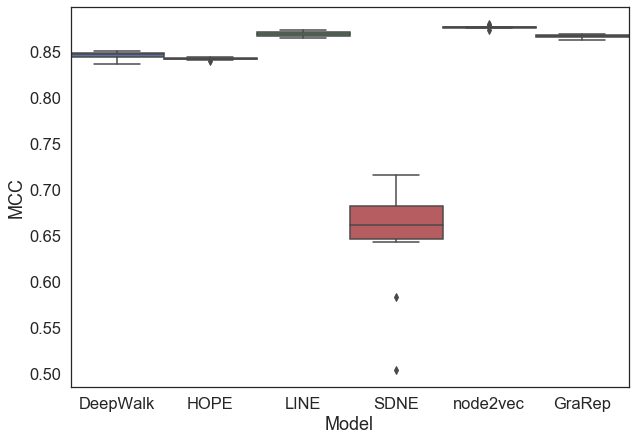
\includegraphics[scale=0.5]
    {figures/boxplot.png}
    \caption[Boxplot of the robustness of NRL models]{\label{fig:boxplot} A boxplot showing the MCC of each NRL model, with the best hyperparameters, repeated ten times to test their robustness.}
\end{figure}

\section{Interpretation of Model Predictions}

Node2vec final embeddings and logistic regression model were trained using the complete graph and exported to be used for predictions. The predictions were created by enquiring the name or identifier of a certain entity. Furthermore, the type of entities to be predicted could also be specified. Three types of relations could be predicted using the model, drug-phenotype, drug-target, or target-phenotype. For each relation predicted the p-value and \ac{MLP} value were calculated and presented. Since methods for drug-target associations, or drug target identification, are well developed, those association results were omitted from the interpretations. To validate the new predictions of the model, positive controls were also presented for drug-phenotype associations.

\subsection{Predicting the Phenotypes for a Drug}
Predicting indications and side effects of a chemical is one of the most common types of tasks used with side effects networks. Table \ref{tab:drug_phenotype} presents the top ten predicted phenotypes for the antipsychotic drug, olanzapine.

\begin{table}[!ht]
    \centering
    \begin{tabular}{|l|l|l|r|r|} 
        \hline
        \textbf{Namespace} & \textbf{Identifier} & \textbf{Name} & \textbf{$p$-value} & \textbf{MLP} \\
        \hline
        umls & C0006384 & Bundle branch block & 0.000 & 3.475 \\
        \hline
        umls & C0575090 & Balance disorder & 0.000 & 3.539 \\
        \hline
        umls & C0878544 & Cardiomyopathy & 0.001 & 2.918 \\
        \hline
        umls & C0233794 & Memory impairment & 0.001 & 2.870 \\
        \hline
        umls & C0004239 & Atrial flutter & 0.001 & 3.297 \\
        \hline
        umls & C0160390 & Liver injury & 0.001 & 3.175 \\
        \hline
        umls & C0020676 & Hypothyroidism & 0.001 & 2.911 \\
        \hline
        umls & C0002884 & Hypochromic anaemia & 0.001 & 3.059 \\
        \hline
        umls & C0034069 & Pulmonary fibrosis & 0.001 & 2.901 \\
        \hline
        umls & C0233477 & Dysphoria & 0.001 & 3.066 \\
        \hline
    \end{tabular}
    \caption{Top phenotypic predictions for olanzapine}
    \label{tab:drug_phenotype}
\end{table}

Olanzapine is an atypical antipsychotic drug that primarily acts on dopamine and serotonin receptors, and is used to treat schizophrenia and bipolar disorders \cite{thomas_olanzapine_2019}. A couple of case reports have presented cardiovascular problems that are associated with olanzapine treatement, one report mentioned that a patient treated with olanzapine experienced bundle branch block, which is a blockage or delay in electrical impulses of the heart \cite{ninan_case_2017}. Another case report presented a patient that suffered from cardiomyopathy after being treated with olanzapine \cite{puttegowda_olanzapine_2016}. Both phenotypes have been predicted with the model, and Figure \ref{fig:olanzapine_phenotypes} shows a subgraph representing some of the paths that are present in the network between olanzapine and three different predicted phenotypes, bundle branch block, cardiomyopathy and balance disorder, which indicate that the predictions could have been made from side-effect similarities.

Studies have been done to investigate the effect of olanzapine, among other atypical antipsychotics, on cognitive function, including attention, memory and verbal learning and they have confirmed that olanzapine improves those cognitive functions in schizophrenia patients \cite{mcgurk_cognitive_2004, smith_effects_2001, cuesta_effects_2001, purdon_neuropsychological_2000, bilder_neurocognitive_2002}. The effect of antipsychotic drugs on the liver has also been studied and it was found that olanzapine can induce hepatic damage \cite{lv_antipsychotic_2018}. Both association with memory and liver injury were predicted using the model. Positive controls, presented in Table \ref{tab:ps_olanzapine} 

\begin{figure}[h!]
    \centering
    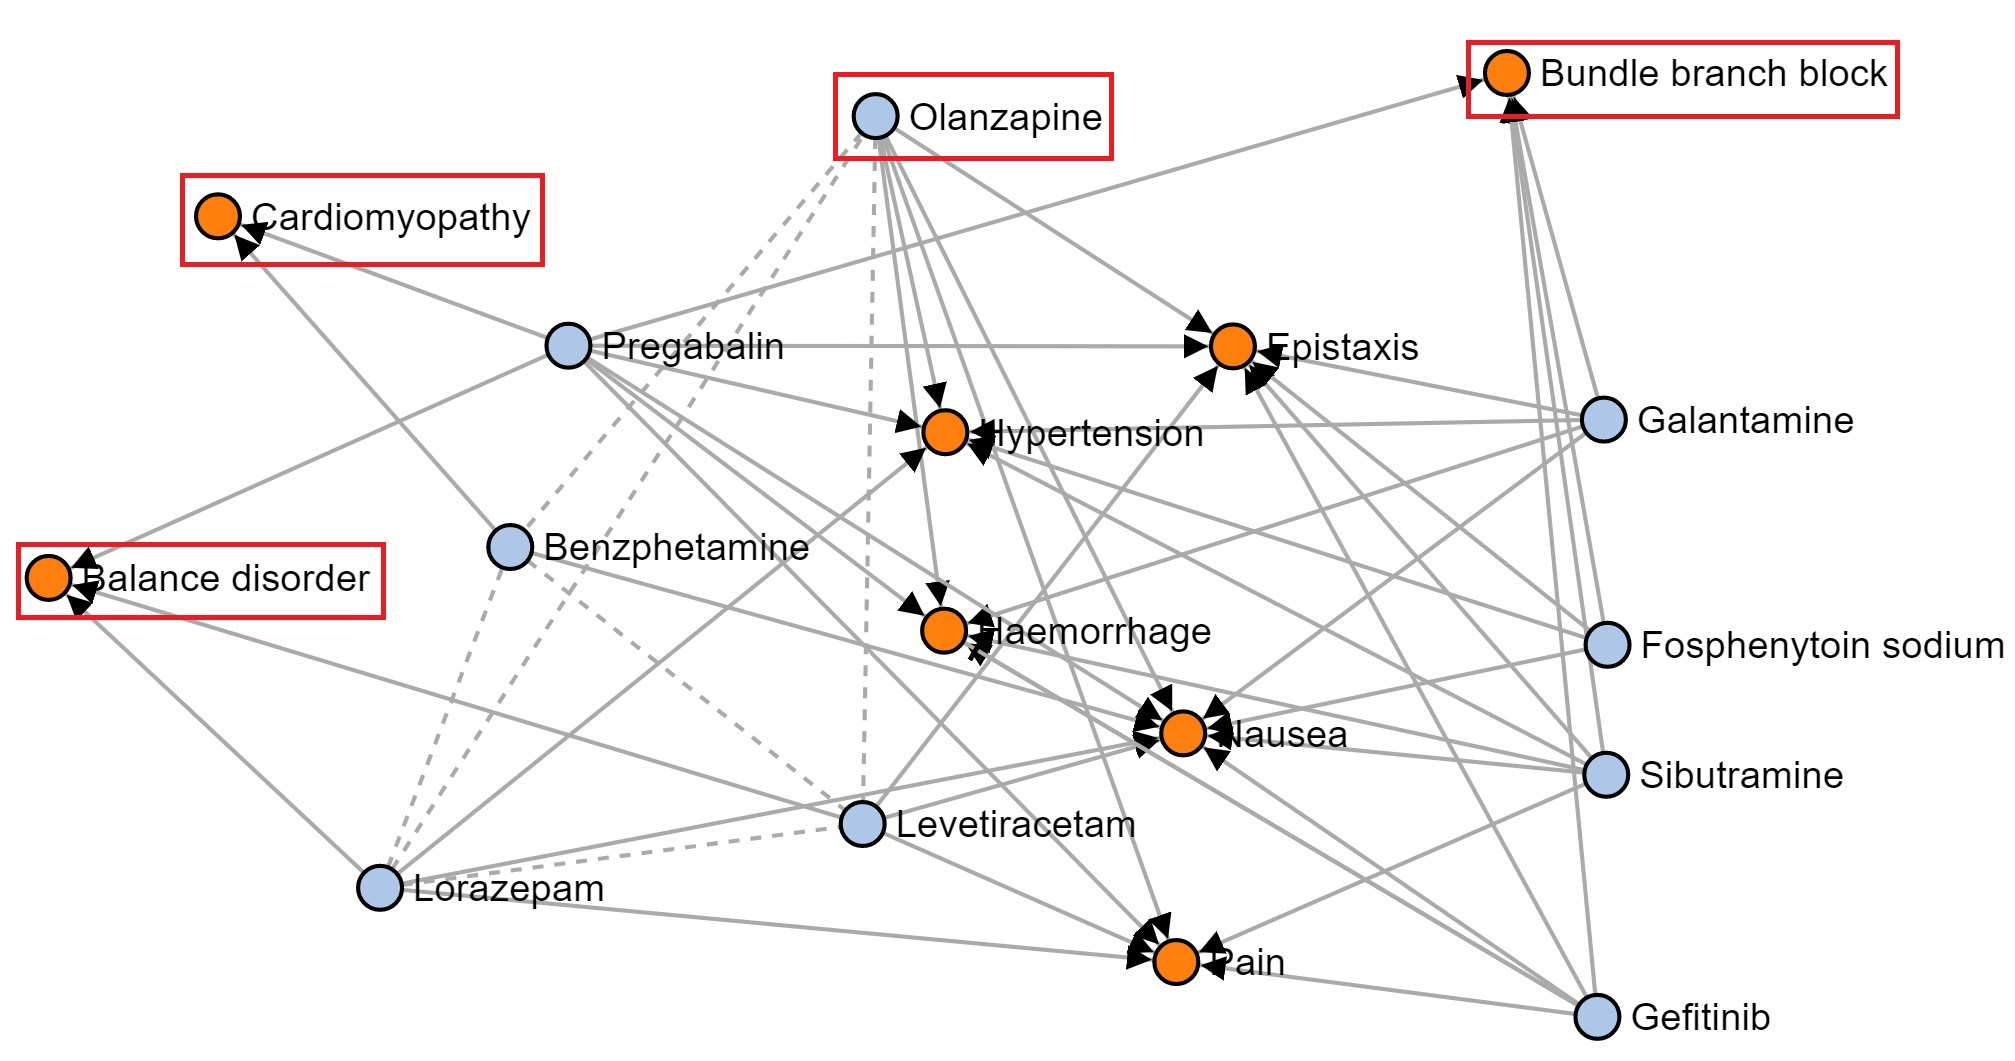
\includegraphics[scale=0.6]
    {figures/olanzapine_phenotypes.jpg}
    \caption[Olanzapine-phentypes path subgraph]{\label{fig:olanzapine_phenotypes} A subgraph showing some of the shortest relation paths between olanzapine and the top three phenotypic predictions}
\end{figure}

\begin{table}
    \centering
    \begin{tabular}{|l|l|l|r|r|}
        \hline
        \textbf{Namespace} & \textbf{Identifier} & \textbf{Name} & \textbf{$p$-value} & \textbf{MLP} \\
        \hline
        umls & C1320474 & Nuchal rigidity &  0.0 & 3.318 \\
        \hline
        umls & C0002453 &  Amenorrhoea &  0.0 & 3.619 \\
        \hline
        umls & C0011168 &  Dysphagia &  0.0 & 3.408 \\
        \hline
        umls &  C0033117 & Priapism &  0.0 &  3.515 \\
        \hline
    \end{tabular}
    \caption{Positive control for olanzapine phenotypic predictions}
    \label{tab:ps_olanzapine}
\end{table}


\subsection{Predicting the Drugs for a Phenotype}
The model can also be used to predict chemicals that can be associated with phenotypes. Here, it used to predict chemicals that might best affect \ac{PD}. 
\ac{PD} is a progressive neurodegenerative disorder that affects motor and non-motor functions in variable degrees \cite{jankovic_parkinsons_2008}. Common motor features of \ac{PD} are tremor, rigidity, slowness (bradykinesia) and impaired balance, other PD symptoms include cognitive impairment and abnormal neurological behaviours \cite{jankovic_parkinsons_2008}. The top ten predictions of chemicals associated with \ac{PD} are shown in Table \ref{tab:phenotype_drug}.

\begin{table}[h]
    \centering
    \begin{tabular}{|l|l|l|r|r|} 
        \hline
        \textbf{Namespace} & \textbf{Identifier} & \textbf{Name} & \textbf{$p$-value} & \textbf{MLP} \\
        \hline
        pubchem.compound &  146570 &  Escitalopram &  0.000 &  3.315 \\
        \hline
        pubchem.compound & 5002 &  Quetiapine &  0.001 &  2.883 \\
        \hline
        pubchem.compound &  5486971 &  Pregabalin &  0.001 &  3.111 \\
        \hline
        pubchem.compound & 68617 &  Sertraline &  0.002 &  2.763 \\
        \hline
        pubchem.compound &  5719 &  Zaleplon &  0.002 &  2.807 \\
        \hline
        pubchem.compound & 60853 & Ziprasidone HCL &  0.002 &  2.613 \\
        \hline
        pubchem.compound & 3345 & Fentanyl &  0.002 &  2.630 \\
        \hline
        pubchem.compound & 5210 & Sibutramine &  0.002 &  2.613 \\
        \hline
        pubchem.compound & 44602 &  Arbaclofen &  0.003 &  2.554 \\
        \hline
        pubchem.compound & 154101 & Dexmethylphenidate &  0.003 &  2.475 \\
        \hline
    \end{tabular}
    \caption{Top chemicals predictions for Parkinson's disease}
    \label{tab:phenotype_drug}
\end{table}

The prediction with the highest significance is escitalopram, a \ac{SSRI} and an $S$-enantiomer of citalopram that is used to treat major depression \cite{weintraub_escitalopram_2006}. Depression is a common complication of \ac{PD}; approximately 20\% to 40\% of \ac{PD} patients have depression and usually the antidepressant treatment of choice is an \ac{SSRI} \cite{weintraub_escitalopram_2006}. Though the efficacy of \ac{SSRI}s on depression in \ac{PD} has not been proven, some studies have found that they could be beneficial \cite{rampello_ssri_2002, hauser_sertraline_1997, ceravolo_paroxetine_2000, menza_citalopram_2004}. One of those studies investigated sertraline, which was also predicted by the model, and found it to be useful in treating depression in \ac{PD} \cite{hauser_sertraline_1997}. Another study evaluated citalopram and found that it can improve the depression symptoms of PD patients \cite{menza_citalopram_2004}. Escitalopram was also investigated and it was concluded that it may be a viable treatment for depression in PD, however more research needs to be conducted to confirm \cite{weintraub_escitalopram_2006, verma_efficacy_2012}. Escitalopram had many paths leading to its association with \ac{PD}, these paths were mostly created from side-effect similarities and target similarities between escitalopram and chemicals that are directly associated with \ac{PD}. Figure \ref{fig:parkinson_escitalopram} shows some of the paths that were found in the network.

\begin{figure}[h!]
    \centering
    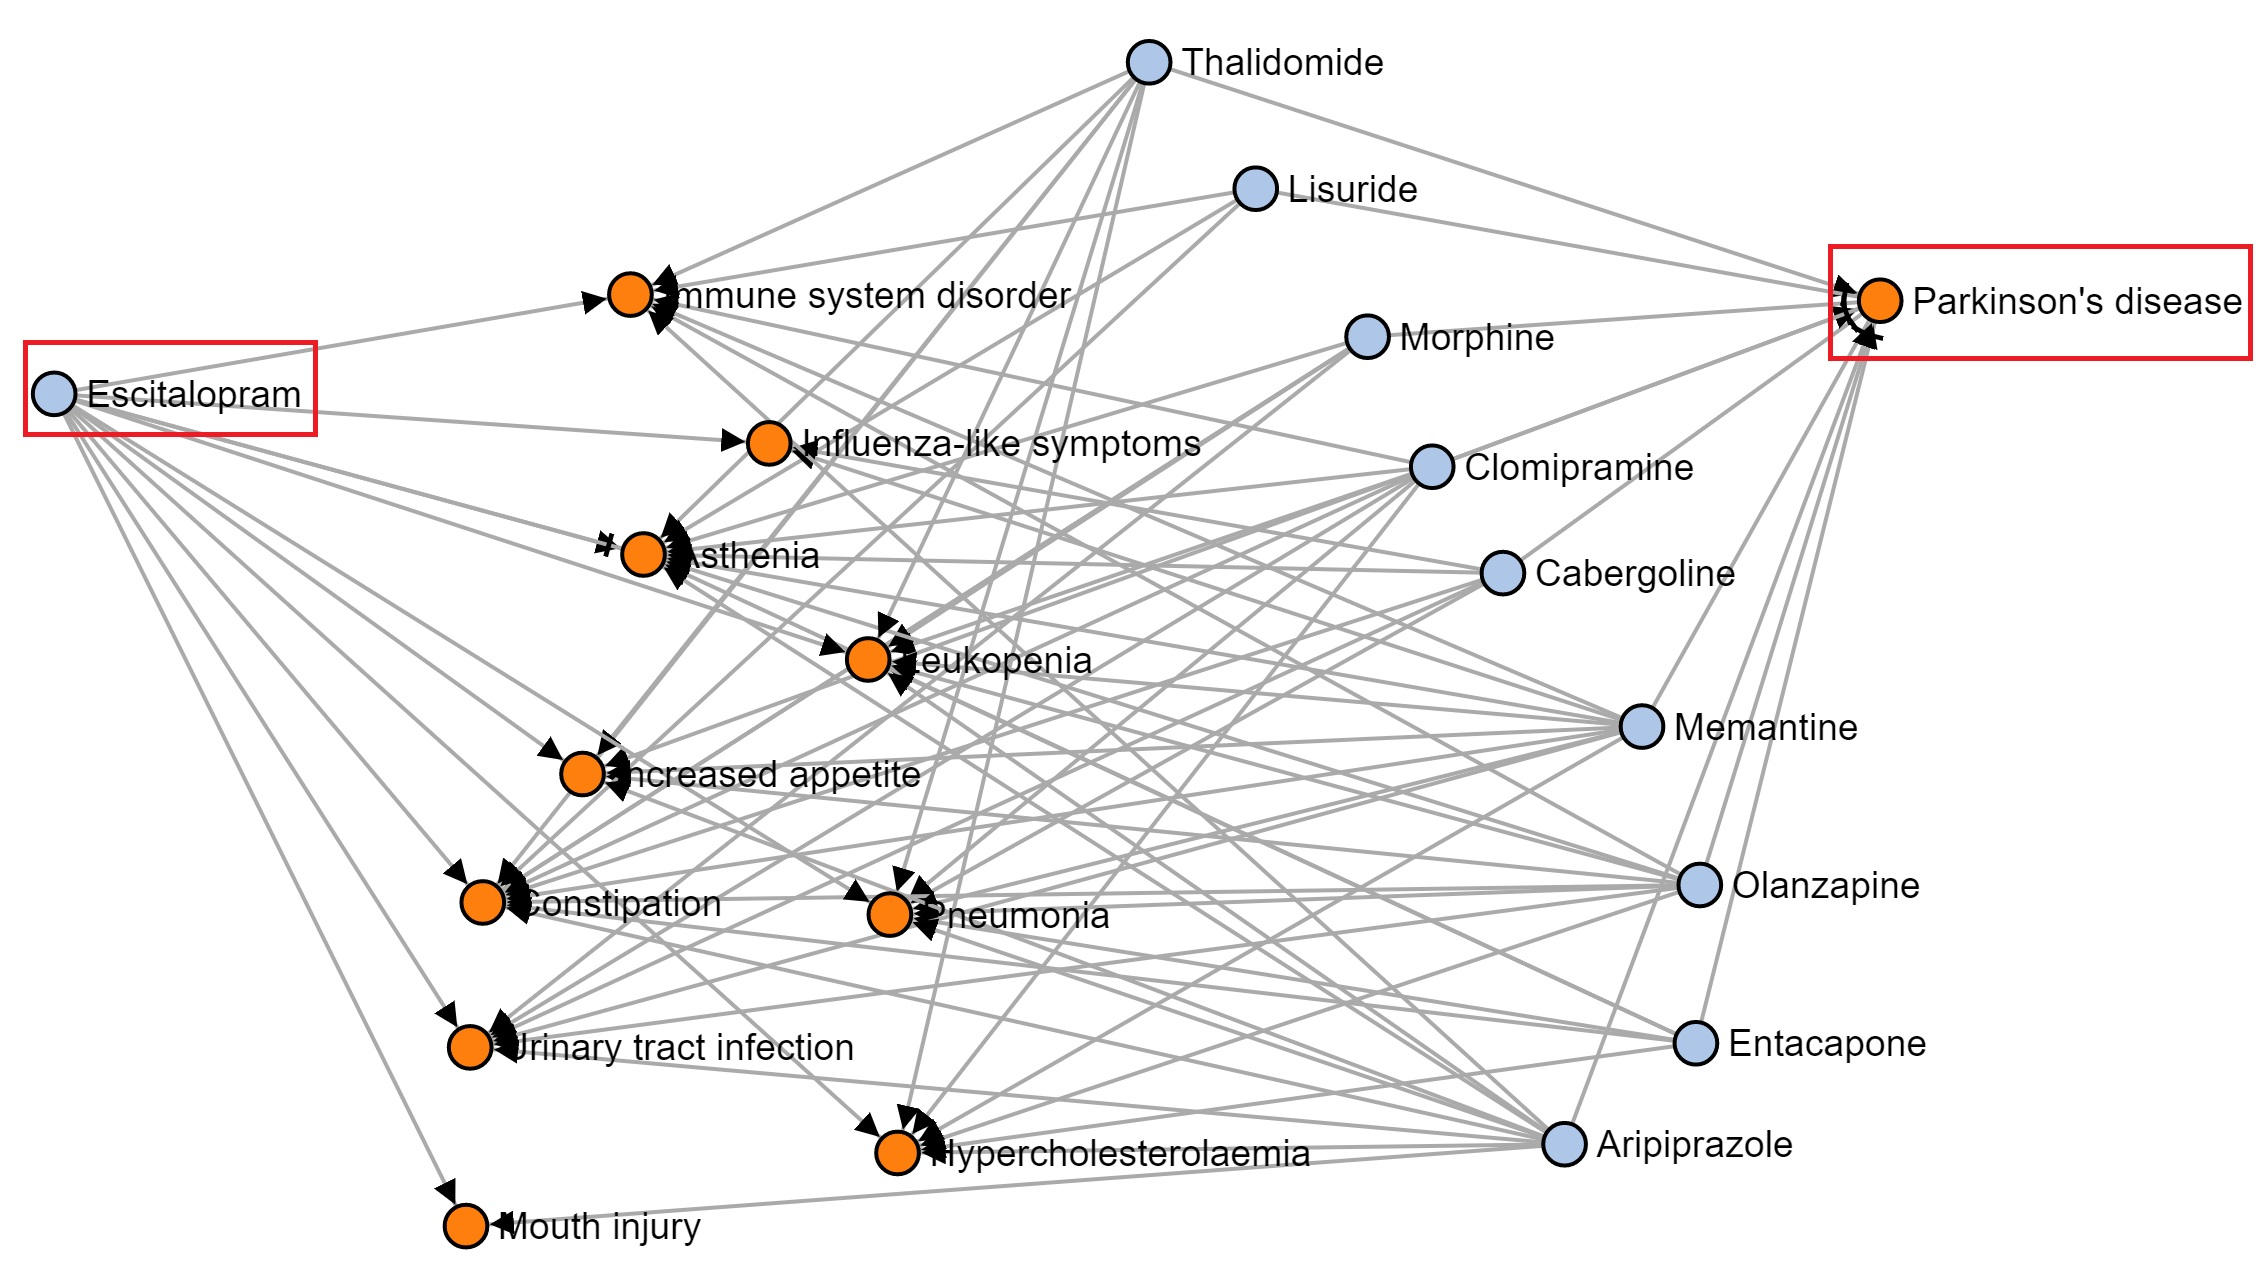
\includegraphics[scale=0.6]
    {figures/parkinson_escitalopram.jpg}
    \caption [Escitalopram-PD path subgraph]{\label{fig:parkinson_escitalopram} A subgraph showing some of the shortest relation paths between escitalopram and \ac{PD}}
\end{figure}

Quetiapine is an antipsychotic drug that has been used to treat schizophrenia and bipolar disorders. It is also used in off-label cases such as post-traumatic stress disorder, anxiety disorders, insomnia, and depression in Parkinson’s disease \cite{el-saifi_quetiapine_2016}, since SIDER is curated from drug labels, this kind of off-label use would not be in the training set. Many researches have investigated quetiapine for treating psychotic symptoms in \ac{PD}, which include delirium, hallucinations, depression, and insomnia among other psychiatric manifestations \cite{desmarais_quetiapine_2016}. Even though those studies have not been able to prove the efficacy of quetiapine on \ac{PD}, they suggest that the high dropout rate might have influenced the results and follow-up studies with larger sample size are required. Figure \ref{fig:parkinson_quetiapine} shows some of the paths in the network that were used to predict the association of quetiapine with \ac{PD}. It is evident from the figure that quetiapine share targets and chemical similarities with two chemicals, bromocriptine and memantine, that are directly associated with \ac{PD}. It is worth mentioning that the prediction of associtation between quetiapine and \ac{PD} was quiet consistent, appearing in the top 30 predictions with different predictive models (not shown). 

\begin{figure}[h!]
    \centering
    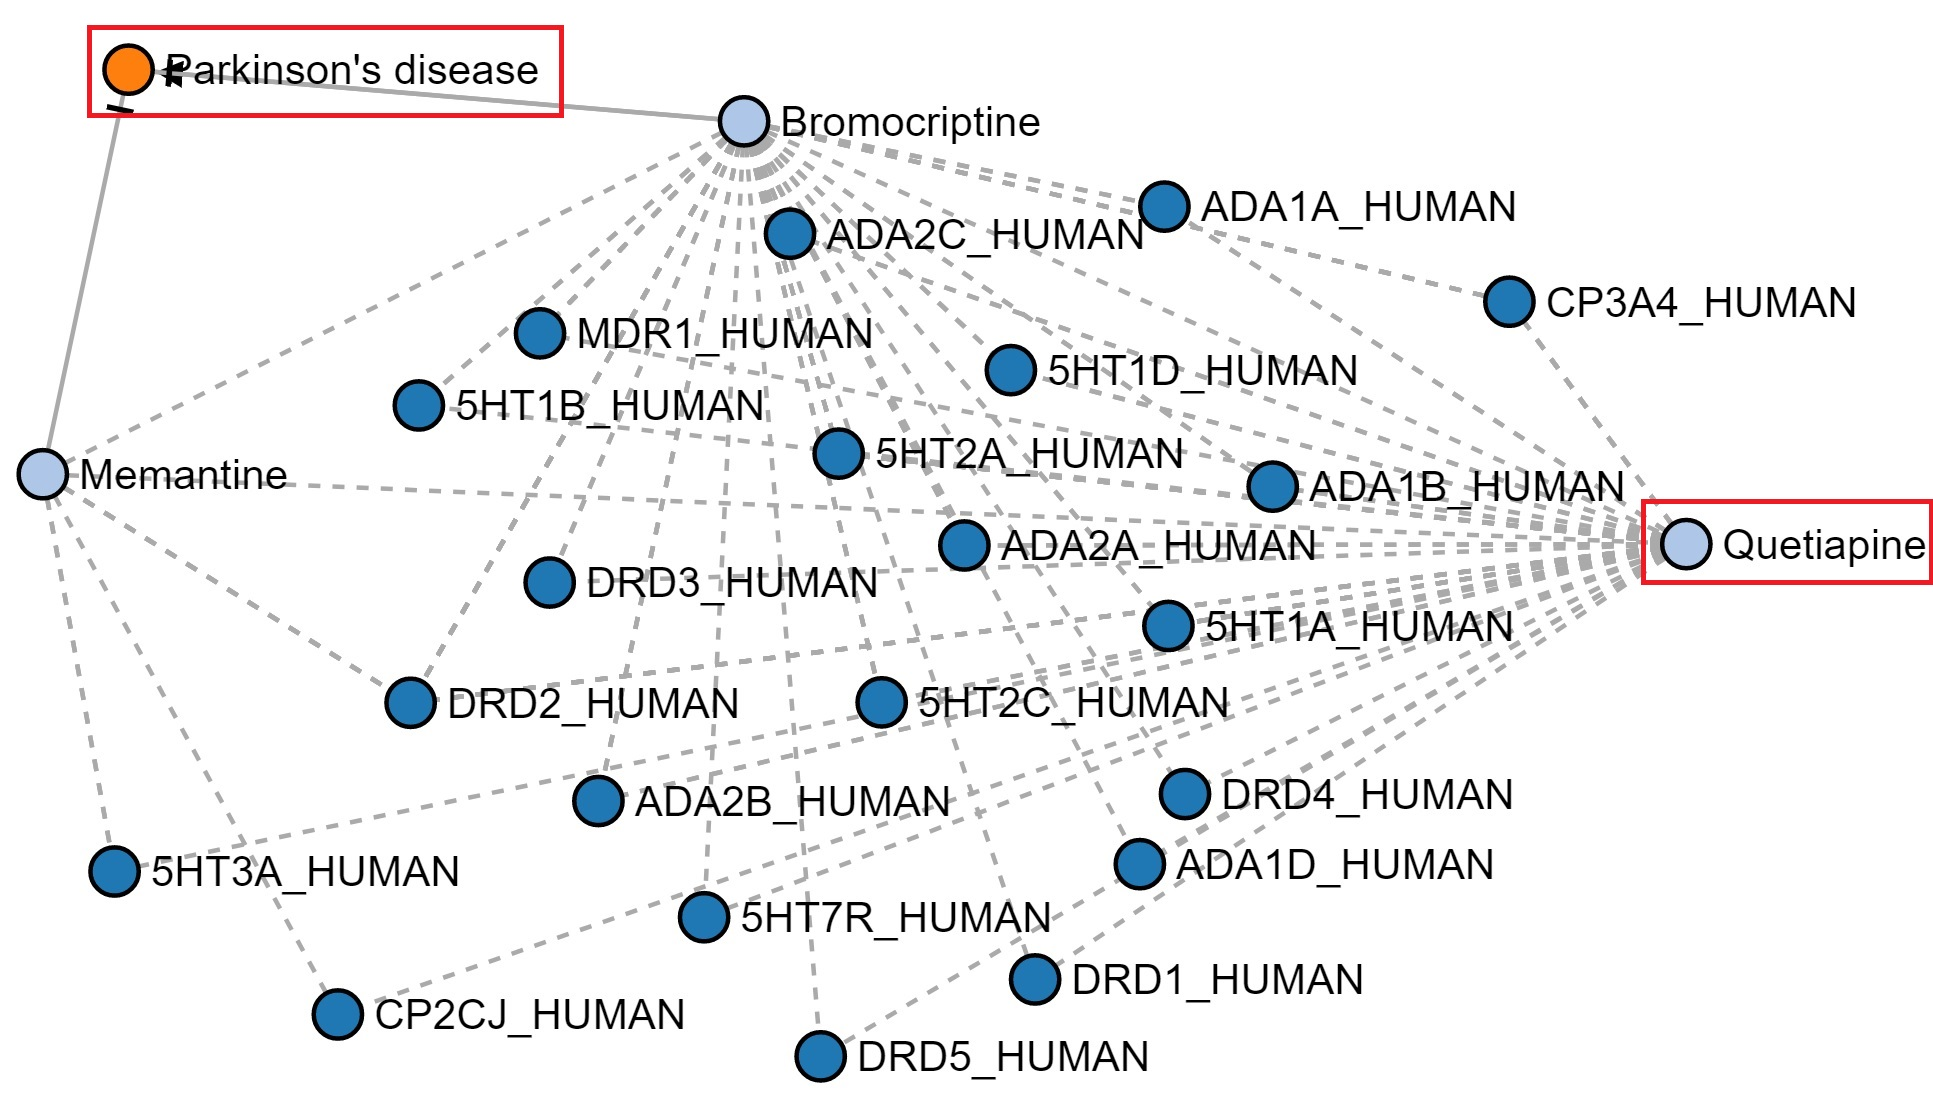
\includegraphics[scale=0.6]
    {figures/parkinson_quetiapine.jpg}
    \caption[Quetiapine-PD path subgraph]{\label{fig:parkinson_quetiapine} A subgraph showing the shortest relation paths between quetiapine and \ac{PD}.}
\end{figure}

A couple of the other predicted chemicals, pregabalin and ziprasidone, have been shown to cause or worsen symptoms of \ac{PD} \cite{perez_lloret_pregabalin-induced_2009, younce_systematic_2019}, while the rest of them do not have any studies that prove their association with \ac{PD}. The positive controls for this association are shown in Table \ref{tab:ps_PD}. These four drugs, selegiline, aripiprazole, ropinirole and clomipramine are already used for treating \ac{PD} and are indicated as such in DrugBank, which is why their association with the disease exists in the network and they are expected to be predicted by the model.

\begin{table}
\centering
\begin{tabular}{|l|l|l|r|r|}
\hline
 \textbf{Namespace} & \textbf{Identifier} & \textbf{Name} & \textbf{$p$-value} & \textbf{MLP} \\
\hline
pubchem.compound & 26757 & Selegiline & 0.001 & 2.831 \\
\hline
pubchem.compound & 60795 &  Aripiprazole &  0.001 &  2.856 \\
\hline
pubchem.compound & 5095 & Ropinirole &  0.001 &  2.997 \\
\hline
pubchem.compound & 2801 & Clomipramine &  0.002 &  2.823 \\
\hline
\end{tabular}
 \caption{Positive control for PD chemicals predictions.}
    \label{tab:ps_PD}
\end{table}

\subsection{Predicting the Phenotypes for a Target }
Another way to use the model is to predict the association of targets with phenotypes. Since there are no direct relations between targets and phenotypes in the network, the model depends on the indirect chemical-chemical, chemical-phenotype, and chemical-target relations to predict target-phenotype relations. Table \ref{tab:target_phenotype} presents predicted phenotypes that are associated with muscarinic 2 cholinergic receptor M2 (M2R).

\begin{table}[h]
    \centering
    \begin{tabular}{ |l|l|l|r|r| } 
        \hline
        \textbf{Namespace} & \textbf{Identifier} & \textbf{Name} & \textbf{$p$-value} & \textbf{MLP} \\
        \hline
        umls & C0013384 & Dyskinesia &  0.009 &  2.070 \\
        \hline
        umls & C0015371 & Extrapyramidal disorder &  0.013 &  1.889 \\
        \hline
        umls & C0026837 & Muscle rigidity &  0.015 &  1.811 \\
        \hline
        umls & C0234133 & Extrapyramidal symptoms &  0.022 &  1.649 \\
        \hline
        umls &  C0026961 & Mydriasis &  0.023 &  1.639 \\
        \hline
        umls & C0013144 & Drowsiness &  0.025 &  1.605 \\
        \hline
        umls &  C0085631 & Agitation &  0.025 &  1.597 \\
        \hline
        umls &  C0686347 & Tardive dyskinesia &  0.038 &  1.419 \\
        \hline
        umls &  C0242422 & Parkinsonism &  0.044 &  1.356 \\
        \hline
        umls &  C0235063 & Respiratory depression &  0.053 &  1.273 \\
        \hline
    \end{tabular}
    \caption{Top phenotypic predictions for M2R}
    \label{tab:target_phenotype}
\end{table}

M2R (uniprot entry name: ACM2\textunderscore HUMAN), encoded by CHRM2 gene, is a receptor belonging to the muscarinic receptors subclass, which contains 5 subtypes (M1-M5) \cite{kleinz_chapter_2008}. These receptors are responsible for recognizing the neurotransmitter acetylcholine and are involved in the cholinergic transduction in the central nervous system, basal ganglia, smooth muscles, and other parasympathetic end organs \cite{aronstam_muscarinic_2009}. A recent study has investigated the role of muscarinic receptors in \ac{TD} and concluded that there is an association variations of CHRM2 and \ac{TD} \cite{boiko_pharmacogenetics_2019}. CHRM2 has also been associated with psychiatric and mood disorders such as schizophrenia and depression \cite{drevets_antidepressant_2013, jeon_role_2015, dean_possible_2015}. A common symptom of mood disorders is agitation, which is one of the phenotypes predicted by the model, furthermore, it has been shown that the inhibition of acetylcholine could cause agitation \cite{carlson_physiology_2019}. Figure \ref{fig:chrm2_phenotypes} shows a subgraph containing the shortest paths from three different phenotypes (agitation, drowsiness and \ac{TD}) to M2R, the paths mostly depend on target and phenotype similarities between drugs, under the assumption that if drugs with the same target have the same phenotype, the target could be the cause of the phenotype.

\begin{figure}[h!]
    \centering
    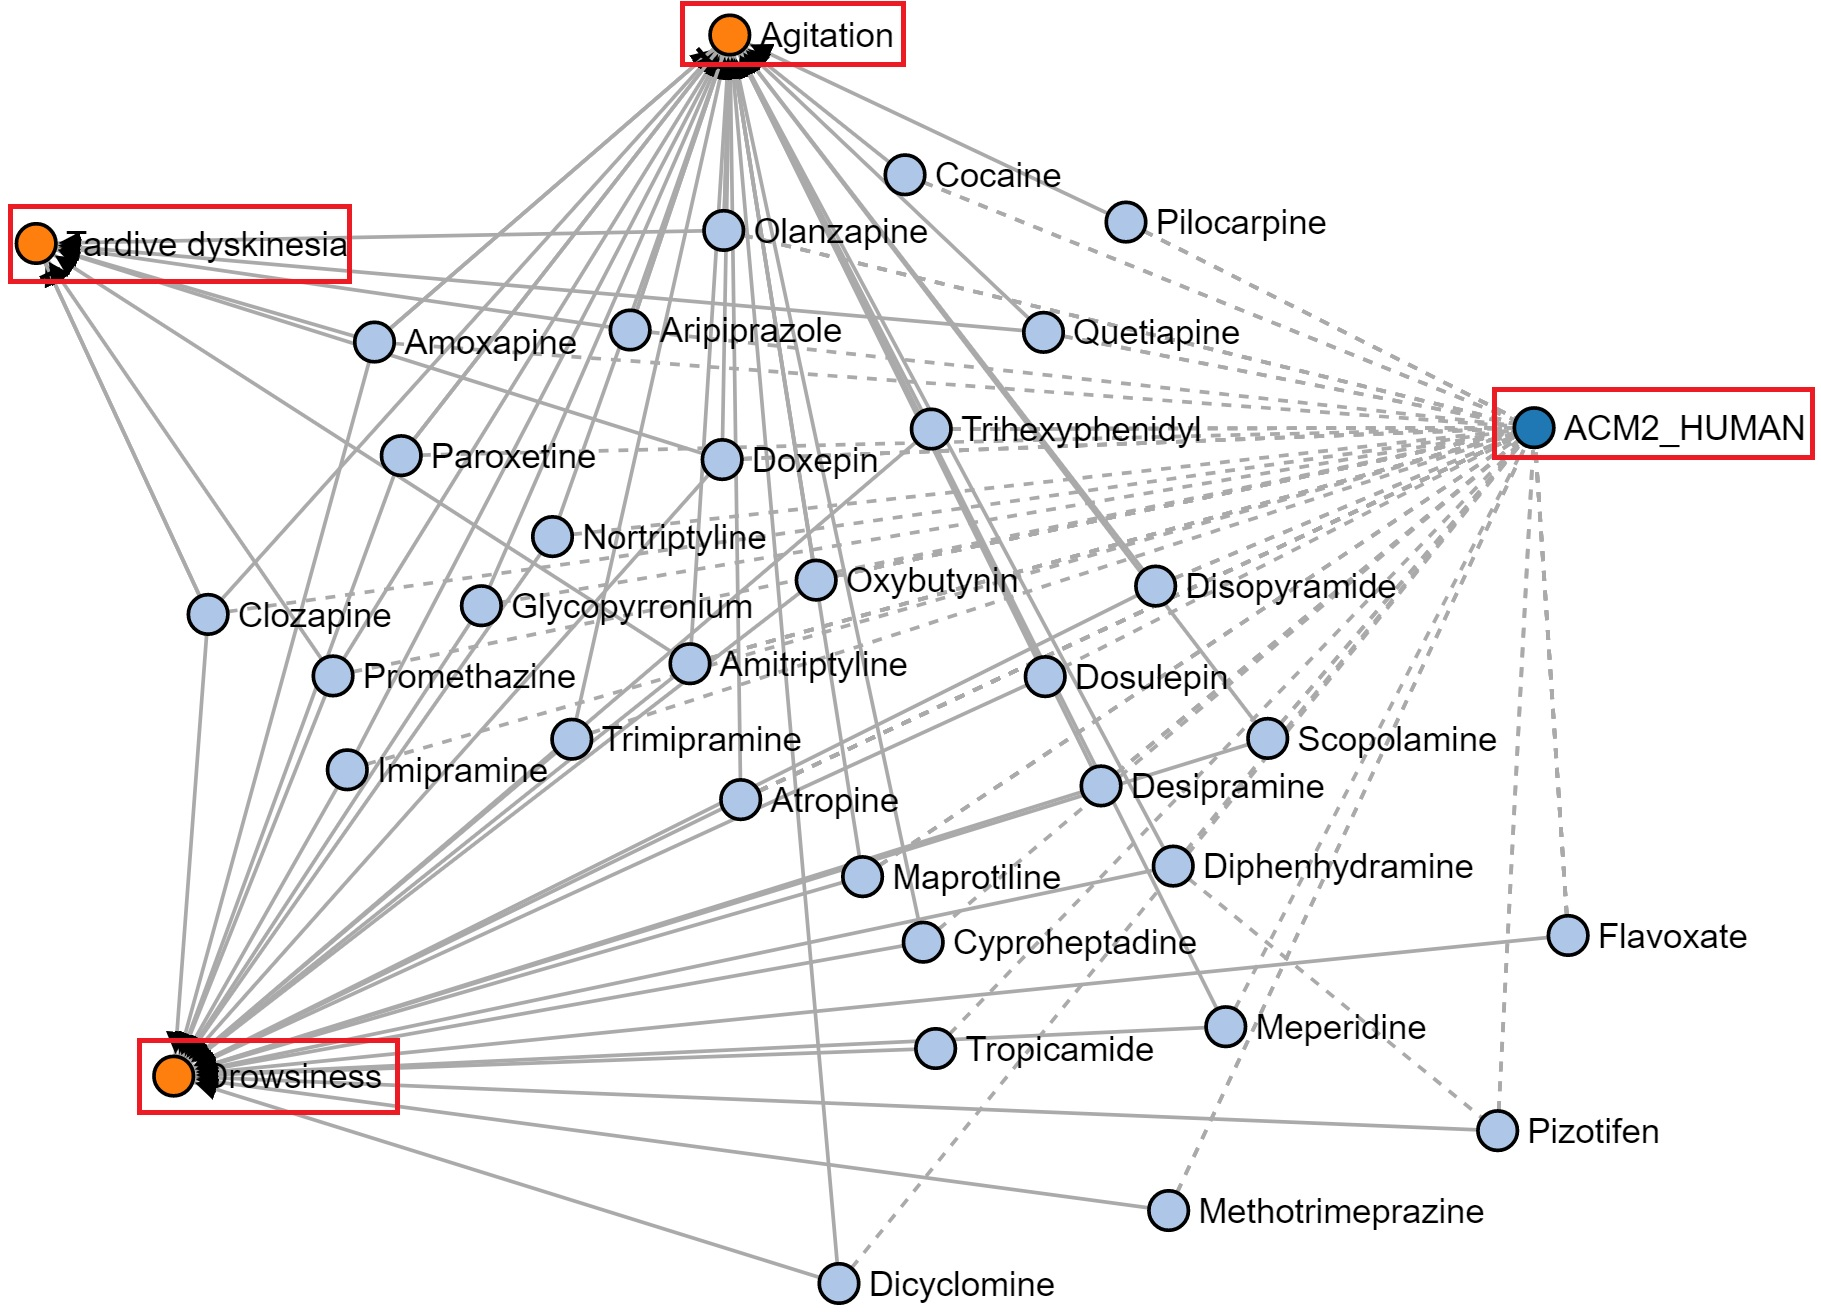
\includegraphics[scale=0.6]
    {figures/chrm2_phenotypes.jpg}
    \caption{\label{fig:chrm2_phenotypes} A subgraph of the shortest paths between M2R (ACM2\textunderscore HUMAN) and three phenotypes (agitation, drowsiness and TD).}
\end{figure}


\section{Reproducibility and Software Implementation}
The scripts and workflows developed in this thesis are available through the seffnet Python package through GitHub at \url{https://github.com/seffnet/seffnet}. Each of its components have been wrapped in a command line interface (CLI) such that the results presented in each section of this work (construction of the network, hyper-parameter optimization, prediction) can be generated with a corresponding command following the guidelines described by Grüning et al. \cite{gruning_software_2019}. 
The seffnet Python package has a tool chain consisting of flake8 (\url{https://github.com/PyCQA/flake8}) to enforce code and documentation quality, setuptools (\url{https://github.com/pypa/setuptools}) to build distributions, pyroma (\url{https://github.com/regebro/pyroma}) to enforce package metadata standards and tox (\url{https://github.com/tox-dev/tox}) as a build tool to facilitate the usage of each of these tools in a reproducible way. It leverages community and open source resources to improve its usability by using Travis-CI (\url{https://travis-ci.com} ) as a continuous integration service.

\section{SEffNet: A Web Application for Link Prediction}
The best machine learning model from the workflow was wrapped with a web application using the Flask Python package (\url{https://github.com/pallets/flask}). It allows users to enter the entity of interest and the types of predictions they want to see (Figure \ref{fig:web_page}) then lists the top results (Figure \ref{fig:protein_prediction}).

\begin{figure}[h!]
    \centering
    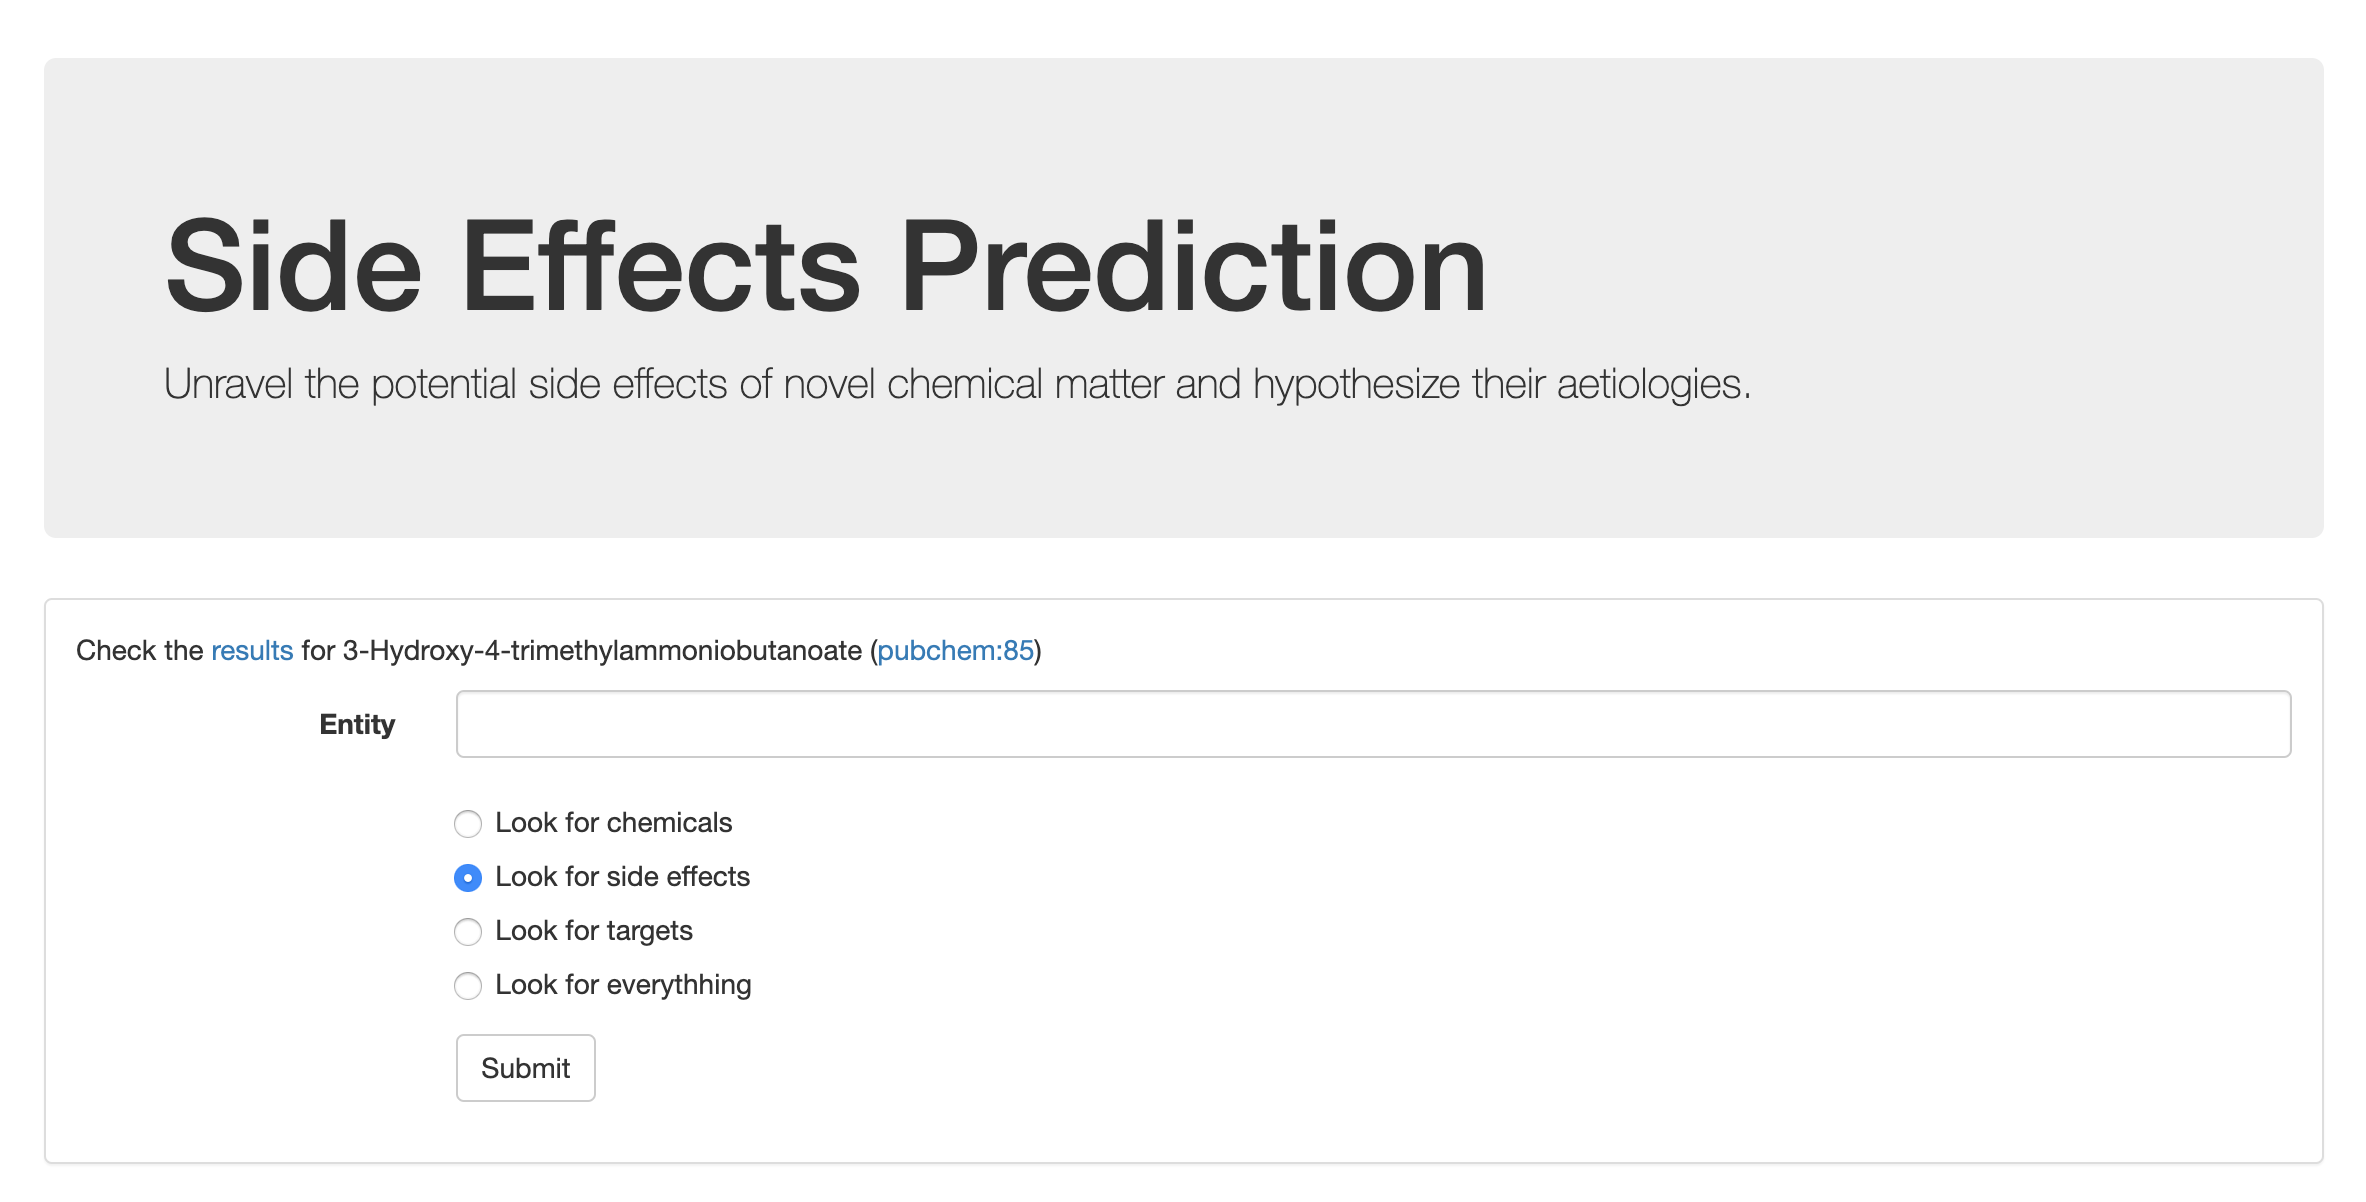
\includegraphics[scale=0.35]
    {figures/web_page.png}
    \caption{\label{fig:web_page} The landing page for the Side Effects Prediction web application.}
\end{figure}

\begin{figure}[h!]
    \centering
    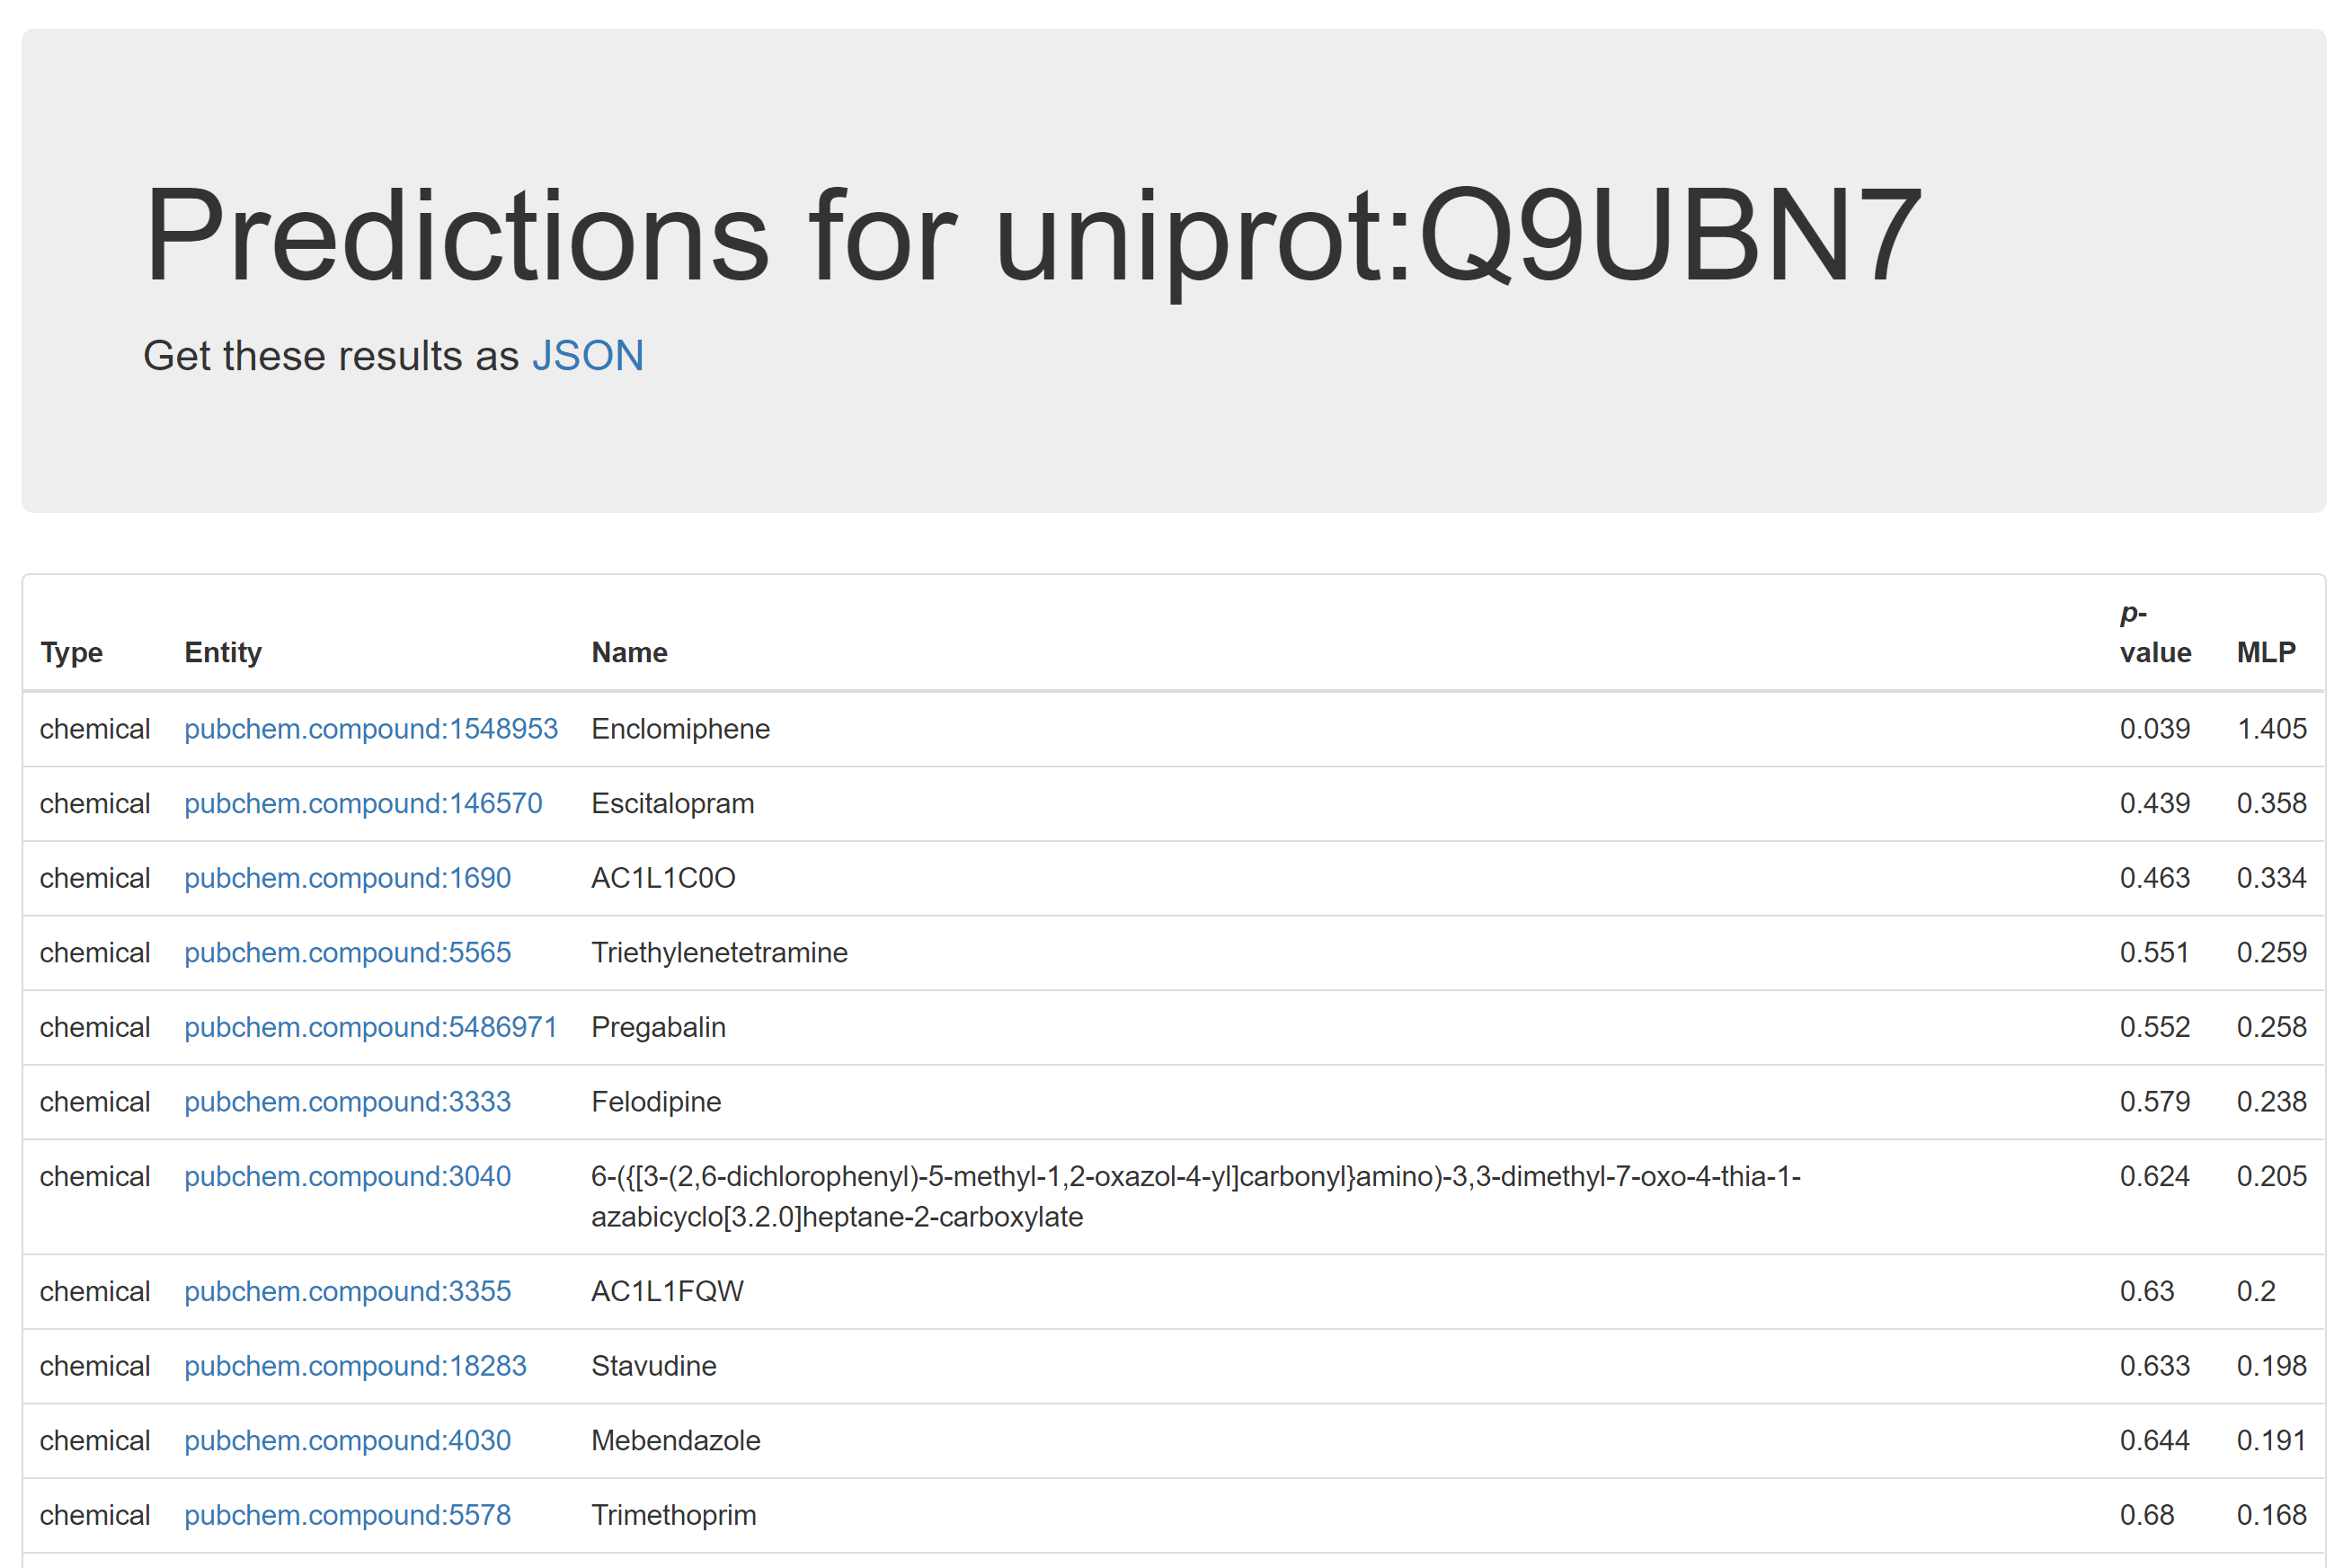
\includegraphics[scale=0.5]
    {figures/protein_prediction.png}
    \caption[The predictions page for chemicals that might interact with HDAC6]{\label{fig:protein_prediction} The predictions page for chemicals that might interact with HDAC6 (uniprot:Q9UBN7), a target of interest in the Human Brain Pharmacome project\footnotemark .}
\end{figure}
\footnotetext{\url{https://pharmacome.scai.fraunhofer.de}}


Because the web application relies on a logistic regression model, predictions are nearly instantaneous. Additionally, the web application also includes an application programming interface (API) that can be used programmatically and incorporated as a microservice in other workflows.
